\documentclass{article}
\usepackage[utf8]{inputenc} %кодировка
\usepackage[T2A]{fontenc}
\usepackage[english,russian]{babel} %русификатор 
\usepackage{mathtools} %библиотека матеши
\usepackage[left=1cm,right=1cm,top=2cm,bottom=2cm,bindingoffset=0cm]{geometry} %изменение отступов на листе
\usepackage{amsmath}
\usepackage{graphicx} %библиотека для графики и картинок
\graphicspath{}
\DeclareGraphicsExtensions{.pdf,.png,.jpg}
\usepackage{subcaption}
\usepackage{pgfplots}
\usepackage{float}
\usepackage{listings}
\usepackage{tikz}


\lstset{
    numbers=left,            % Нумерация строк слева
    numberstyle=\tiny,       % Размер шрифта для номеров строк
    stepnumber=1,            % Нумеровать каждую строку
    numbersep=5pt,           % Расстояние между номерами и кодом
    backgroundcolor=\color{white},  % Цвет фона
    showspaces=false,        % Не показывать пробелы
    showstringspaces=false,  % Не показывать пробелы в строках
    showtabs=false,          % Не показывать табуляцию
    frame=single,            % Рамка вокруг кода
    tabsize=2,               % Размер табуляции
    breaklines=true,         % Автоматический перенос строк
    breakatwhitespace=true   % Переносить строки только по пробелам
}

\begin{document}
% НАЧАЛО ТИТУЛЬНОГО ЛИСТА
\begin{center}
    \Large
    Федеральное государственное автономное \\
    образовательное учреждение высшего образования \\ 
    «Научно-образовательная корпорация ИТМО»\\
    \vspace{0.5cm}
    \large
    Факультет программной инженерии и компьютерной техники \\
    Направление подготовки 09.03.04 Программная инженерия \\
    \vspace{1cm}
    \Large
    \textbf{Отчёт по лабораторной работе №3} \\
        По дисциплине «Системы ввода-вывода» ( семестр 6)\\
    \large
    \vspace{8cm}

    \begin{minipage}{.33\textwidth}
    \end{minipage}
    \hfill
    \begin{minipage}{.4\textwidth}
    
        \textbf{Студент}: \vspace{.1cm} \\
        \ Дениченко Александр P3312\\
        \ Разинкин Александр P3307\\
        \ Балин Артём P3312\\
        \textbf{Практик}:  \\
        \ Табунщик Сергей Михайлович
    \end{minipage}
    \vfill
Санкт-Петербург\\ 2025 г.
\end{center}
\pagestyle{empty}
% КОНЕЦ ТИТУЛЬНОГО ЛИСТА 
\newpage
\pagestyle{plain}

\section*{Цель}
Изучение протоколов передачи данных между устройствами.
Познакомится с принципами обмена данными между
устройствами, алгоритмами обмена и форматами передачи данных на
примере интерфейсов I2C, SPI, 1-Wire.
\section{Задачи}
Написать драйвер символьного устройства, удовлетворяющий
требованиям:

• должен создавать символьное устройство /dev/varN, где N – это
номер варианта

• должен обрабатывать операции записи и чтения в соответствии с
вариантом задания

\section{Вариант}

При записи текста в файл символьного устройства должно
запоминаться количество пробелов во введенном тексте.
Последовательность полученных результатов с момента
загрузки модуля ядра должна выводиться при чтении файла.

\section{Замеры DHT-11}

\begin{center}
  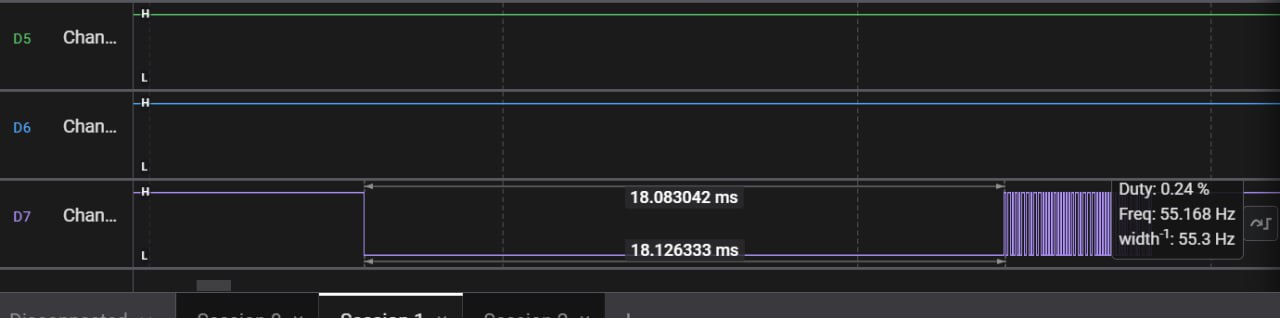
\includegraphics[width=.9\textwidth]{dht-11}
\end{center}
Изначально host опускает линию в 0 на 18 ms. Далее он отпускает для ожидания сигнала ответа от slave и затем slave отпускает линию.
Далее идут данные.

Расшифровка самих данных ТР1: 00011011 00000000 00010111 00000100 00110110.

В конце он отпускает линию.

Расчёты (первая транзакция): 
\begin{itemize}
  \item Humidity = 00011011 00000000 = 27\%
  \item Temp = 00010111 00110110 = 23.015625$C^0$
\end{itemize}

\begin{center}
  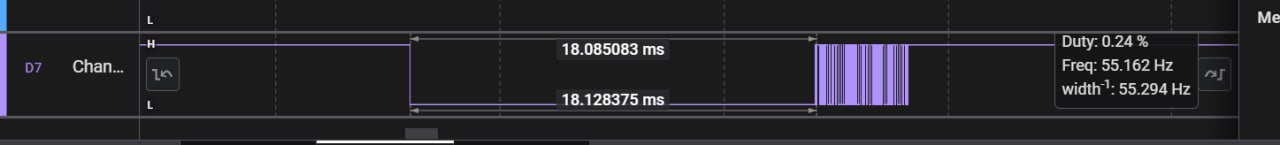
\includegraphics[width=.9\textwidth]{dht-11-2}
\end{center}

Расшифровка самих данных ТР2: 00011011 00000000 00010111 00000100 00110110.

Расчёты (вторая транзакция): 
\begin{itemize}
  \item Humidity = 27\%
  \item Temp = 23.015625$C^0$
\end{itemize}

\begin{center}
  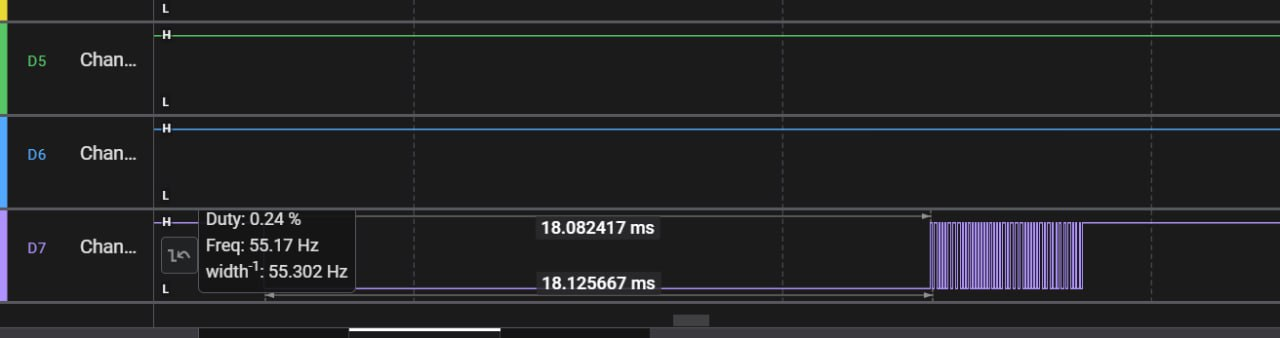
\includegraphics[width=.9\textwidth]{dht-11-3}
\end{center}

Расшифровка самих данных ТР3: 00011100 00000000 00010111 00000101 00111000.

Расчёты (третья транзакция): 
\begin{itemize}
  \item Humidity = 28\%
  \item Temp = 23.019531$C^0$
\end{itemize}

\section{Замеры I2C}

\begin{center}
  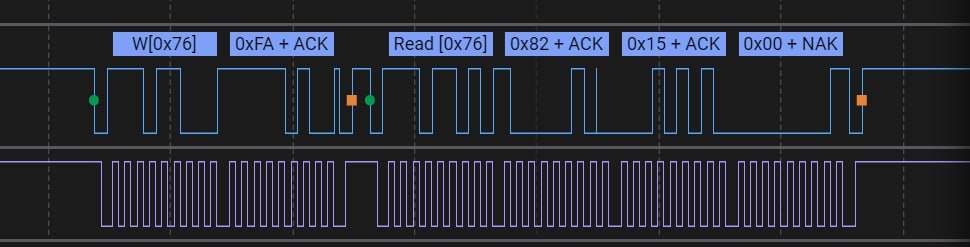
\includegraphics[width=.9\textwidth]{i2c-1}
\end{center}

Изначально передаётся write сигнал с номером устройства и номером регистра для чтения из необходимого slave сигнал.


\begin{center}
  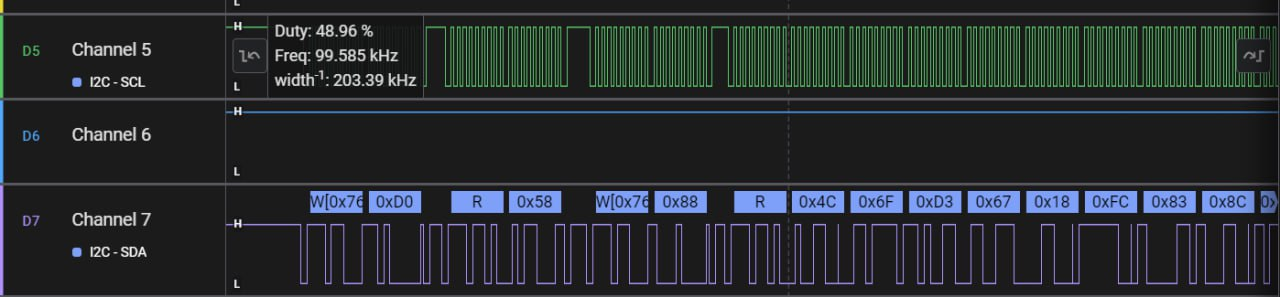
\includegraphics[width=.9\textwidth]{i2c-2}
\end{center}

\begin{lstlisting}[caption={main.py}, label={lst:example}]
  def get_temperature():
    adc_T = 0x82150  
    dig_T1 = 28492
    dig_T2 = 26579
    dig_T3 = -1000

    var1 = (((adc_T >> 3) - (dig_T1 << 1)) * dig_T2) >> 11
    var2 = (((((adc_T >> 4) - dig_T1) * ((adc_T >> 4) - dig_T1)) >> 12) * dig_T3) >> 14

    t_fine = var1 + var2

    T = (t_fine * 5 + 128) >> 8

    return T / 100.0  

  temperature = get_temperature()
  print(f"{temperature:.2f}")

\end{lstlisting}


\[
dig_{T1} = 28492\ 
dig_{T2} = 26579\
dig_{T3} = -1000\
\]


Температура (транзакция превая) -- 24.31


\begin{center}
  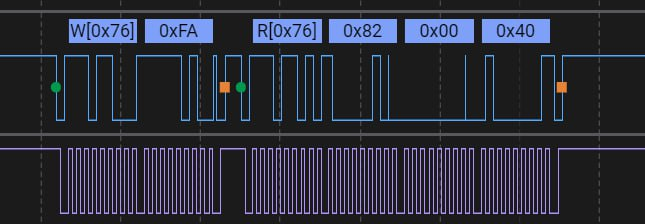
\includegraphics[width=.9\textwidth]{i2c-3.jpg}
\end{center}

Температура (транзакция вторая, третья) -- 24.21


\section{Эмуляция сигнала вручную single wire}


\begin{center}
  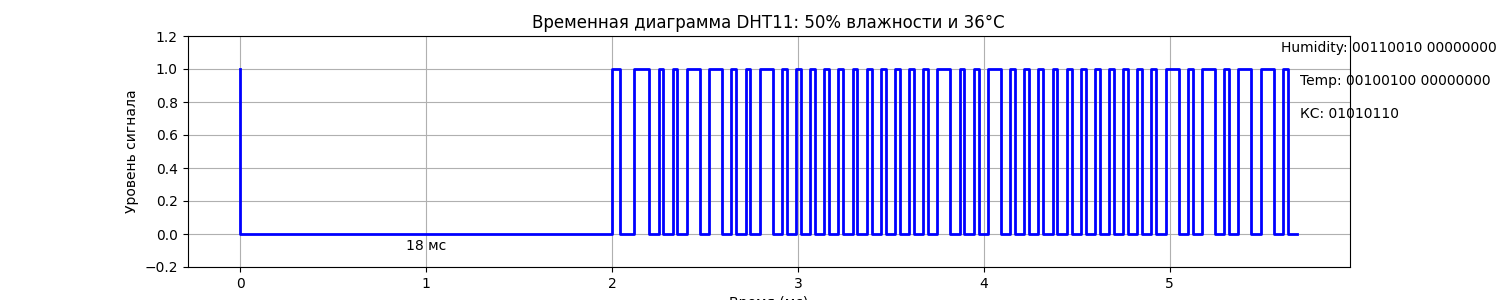
\includegraphics[width=.9\textwidth]{handmadedh.png}
\end{center}

\section{Эмуляция сигнала вручную I2C}
\begin{center}
  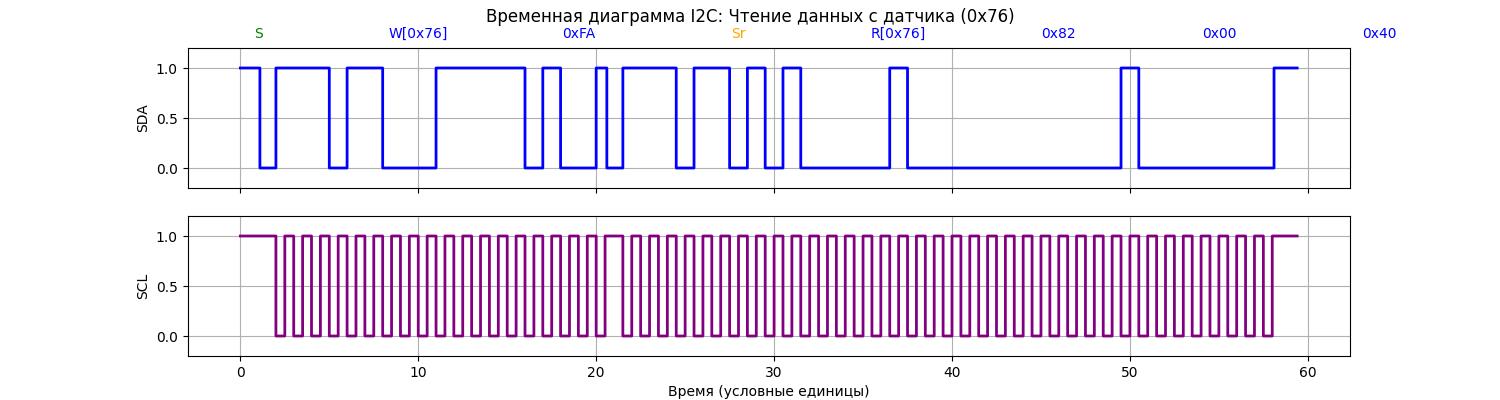
\includegraphics[width=.9\textwidth]{i2c_diagram_updated.png}
\end{center}

\section{Определение скорости }
Single wire: 

Скорость передачи данных составляет примерно 12 109 бит/с или же 12.1 кбит/с.
\\ \\
I2C: 

Скорость передачи данных составляет примерно 187 501 бит/с или же  187.5 кбит/с.


\end{document}
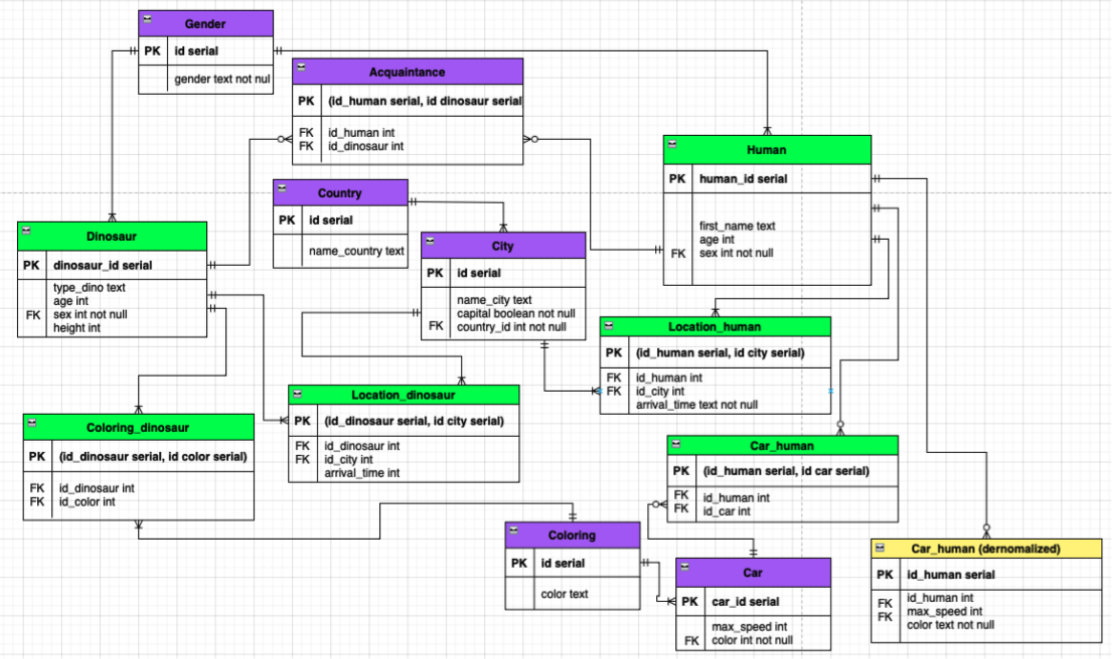
\includegraphics[width=.9\textwidth]{123}
\begin{lstlisting}[caption={kernel.ld}, label={lst:example}]
    
\end{lstlisting}
